% !TEX program = xelatex
% !TEX encoding = UTF-8
% ============================================
% 数学笔记 XeLaTeX 模板 v0.0.1
% 基于现有数学笔记的结构和风格
% ============================================

\documentclass[a4paper, 11pt]{ctexart}

% ============================================
% 包的引入
% ============================================

% 数学公式与符号
\usepackage{amsmath, amssymb, amsthm, amsfonts}
\usepackage{mathtools} % 增强的数学工具

% 页面设置
\usepackage{geometry}
\geometry{left=2cm, right=2cm, top=2.5cm, bottom=2.5cm}

% 颜色支持
\usepackage{xcolor}

% 绘图支持
\usepackage{tikz}
\usetikzlibrary{arrows.meta, positioning, intersections, quotes, calc}

% 彩色文本框
\usepackage[most]{tcolorbox}

% 超链接
\usepackage[colorlinks=true, linkcolor=myblue, citecolor=mygreen, urlcolor=myred]{hyperref}

% 图片支持
\usepackage{graphicx}

% 其他工具
\usepackage{caption} % 支持 \captionof 命令
\usepackage{enumitem} % 增强的列表环境
\usepackage{microtype} % 更好的文字微调
\usepackage{fancyhdr} % 页眉页脚
\usepackage{lastpage} % 总页数引用

% ============================================
% 颜色定义(兼容黑白打印)
% ============================================
\definecolor{myblue}{RGB}{0, 112, 192}
\definecolor{mygreen}{RGB}{0, 176, 80}
\definecolor{myorange}{RGB}{247, 150, 70}
\definecolor{myred}{RGB}{200, 0, 0}
\definecolor{mypurple}{RGB}{152, 78, 163}
\definecolor{mygray}{gray}{0.95}

% ============================================
% 全局排版与辅助命令
% ============================================
\linespread{1.2}
\setlength{\parindent}{0pt}
\setlength{\parskip}{0.6em}
\setlength{\headheight}{14pt}
\setlist[itemize]{leftmargin=1.7em}
\setlist[enumerate]{leftmargin=1.9em}
\numberwithin{equation}{section}

\newcommand{\notetitle}{数学笔记标题}
\newcommand{\noteauthor}{作者姓名}
\newcommand{\notedate}{\today}

% 常用数学集合与符号
\newcommand{\R}{\mathbb{R}}
\newcommand{\C}{\mathbb{C}}
\newcommand{\Q}{\mathbb{Q}}
\newcommand{\Z}{\mathbb{Z}}
\newcommand{\N}{\mathbb{N}}
\newcommand{\dd}{\mathop{}\!\mathrm{d}}
\DeclarePairedDelimiter{\abs}{\lvert}{\rvert}
\DeclarePairedDelimiter{\norm}{\lVert}{\rVert}

% 关键词高亮
\newcommand{\keyword}[1]{\textcolor{myorange}{\textbf{#1}}}

% ============================================
% 定理、定义、例题环境设置
% ============================================

\tcbset{
    mathnote/.style={
        enhanced,
        breakable,
        boxrule=0.8pt,
        colback=#1!5!white,
        colframe=#1!75!black,
        fonttitle=\bfseries,
        top=8mm,
        left=1.2em,
        right=1.2em,
        bottom=1em,
        attach boxed title to top left={xshift=1cm, yshift=-2mm},
        sharp corners,
        boxed title style={
            sharp corners,
            colback=#1!75!black
        }
    }
}

% 定理环境
\newtcolorbox{theorembox}[1]{mathnote=myblue,title=定理:#1}

% 定义环境
\newtcolorbox{definitionbox}[1]{mathnote=mygreen,title=定义:#1}

% 例题/技巧与应用环境
\newtcolorbox{examplebox}[1]{mathnote=myorange,title=技巧与应用:#1}

% 引理环境
\newtcolorbox{lemmabox}[1]{mathnote=mypurple,title=引理:#1}

% 注意/提醒环境
\newtcolorbox{notebox}[1]{mathnote=myred,title=注意:#1,colback=mygray}

% 总结思路环境
\newtcolorbox{summarybox}[1]{mathnote=myblue,title=总结:#1,colback=myblue!3!white}

% ============================================
% 标题格式设置
% ============================================
\usepackage{titlesec}
\titleformat{\section}
    {\Large\bfseries\color{myblue}}
    {\thesection}{1em}{}
\titleformat{\subsection}
    {\large\bfseries\color{myorange}}
    {\thesubsection}{1em}{}

% ============================================
% 数学定理环境(使用 amsthm)
% ============================================
\theoremstyle{definition}
\newtheorem{theorem}{定理}[section]
\newtheorem{definition}{定义}[section]
\newtheorem{lemma}{引理}[section]
\newtheorem{corollary}{推论}[theorem]
\newtheorem{example}{例题}[section]

% ============================================
% 页眉页脚
% ============================================
\pagestyle{fancy}
\fancyhf{}
\fancyhead[L]{\color{myblue}\notetitle}
\fancyhead[R]{\color{myorange}\leftmark}
\fancyfoot[L]{\noteauthor}
\fancyfoot[R]{\thepage/\pageref{LastPage}}
\renewcommand{\headrulewidth}{0.4pt}
\renewcommand{\footrulewidth}{0.4pt}

\fancypagestyle{plain}{%
    \fancyhf{}
    \fancyfoot[L]{\noteauthor}
    \fancyfoot[R]{\thepage/\pageref{LastPage}}
    \renewcommand{\headrulewidth}{0pt}
    \renewcommand{\footrulewidth}{0.4pt}
}

% ============================================
% 文档开始
% ============================================
\begin{document}

% 标题页
\title{\Huge \bfseries \color{myblue} \notetitle}
\author{\noteauthor}
\date{\notedate}
\maketitle

% 目录
\tableofcontents
\newpage

% ============================================
% 正文内容示例
% ============================================

\section{第一部分:基础概念}

\subsection{基本定义}

\begin{definitionbox}{基本概念示例}
这是一个定义环境的示例。你可以在这里放置数学定义、概念说明等内容。

例如:设 $f: \R \to \R$ 是一个函数,若存在常数 $M$ 使得 $\abs{f(x)} \le M$,则称 $f$ 有界。记向量范数 $\norm{\mathbf{v}}_2$ 表示欧几里得范数,积分时使用 $\dd x$ 可以保持格式统一。
\end{definitionbox}

\subsection{重要定理}

\begin{theorembox}{重要定理示例}
这是一个定理环境的示例。你可以在这里放置定理、公式等。

\begin{equation}
    \sin^2\alpha + \cos^2\alpha = 1
\end{equation}
\end{theorembox}

\subsection{应用示例}

\begin{examplebox}{解题技巧示例}
这是一个例题/技巧环境的示例。你可以在这里放置解题方法、技巧说明等。

\textbf{解题步骤:}
\begin{enumerate}
    \item 第一步:\keyword{审题},明确已知与所求;
    \item 第二步:整理公式,必要时写出 $\norm{\cdot}$、$\abs{\cdot}$ 等限制;
    \item 第三步:计算并验证,记录可复用的思路。
\end{enumerate}
\end{examplebox}

% ============================================
% TikZ 绘图示例
% ============================================
\section{图形示例}

\begin{center}
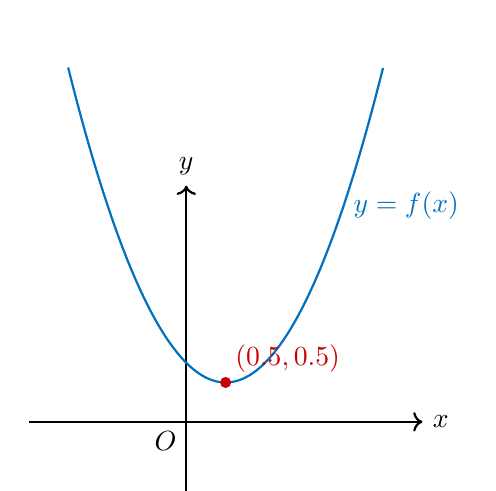
\begin{tikzpicture}[scale=1]
    % 坐标轴
    \draw[->, thick] (-2,0) -- (3,0) node[right] {$x$};
    \draw[->, thick] (0,-1) -- (0,3) node[above] {$y$};
    \node at (0,0) [below left] {$O$};
    
    % 函数图像示例(抛物线)
    \draw[myblue, thick, domain=-1.5:2.5, samples=100] plot (\x, {(\x-0.5)^2 + 0.5});
    \node[myblue, right] at (2, {((2-0.5)^2 + 0.5)}) {$y = f(x)$};
    
    % 标注点
    \fill[myred] (0.5, 0.5) circle (2pt) node[above right] {$(0.5, 0.5)$};
\end{tikzpicture}
\captionof{figure}{函数图像示例}
\end{center}

% ============================================
% 注意事项示例
% ============================================
\section{注意事项}

\begin{notebox}{重要提醒}
这是一个注意事项环境的示例。你可以在这里放置需要特别提醒的内容。
\end{notebox}

\begin{summarybox}{本节要点回顾}
使用盒子环境可以快速整理概念、定理与技巧;页眉页脚会自动带出标题与章节,便于翻阅;常用命令如 $\R,\C,\abs{\cdot},\norm{\cdot}$ 可以保持公式一致性。
\end{summarybox}

% ============================================
% 文档结束
% ============================================
\end{document}



